\begin{frame}{Hello from IRIS-HEP and Scikit-HEP!}
  \begin{columns}
    \column{0.6\textwidth}
    \Large
    % \begin{itemize}
    \begin{itemize}\setlength{\itemsep}{0.5 cm}
      \item We're members of the \href{https://iris-hep.org/}{Institute for Research and Innovation in Software for High Energy Physics (IRIS-HEP)} and \href{https://scikit-hep.org/}{Scikit-HEP} and we're developers of a Pythonic data analysis ecosystem for HEP
      \item Goals: Empower analysts with modern data science stacks and provide powerful libraries for building expressive workflows
    \end{itemize}
%
    \column{0.4\textwidth}
    \begin{figure}
        \begin{center}
            
\includegraphics[width=0.9\linewidth]{iris-hep-logo-long.pdf}
            
\includegraphics[width=0.8\linewidth]{scikit-hep-logo.pdf}
        \end{center}
    \end{figure}
  \end{columns}
\end{frame}

% shows the rapid adoption of Python for analysis in recent years
\begin{frame}{Use of Scientific Python (NumPy, etc.) is somewhat recent to HEP}
\vspace{0.25 cm}
\textcolor{darkblue}{Source: ``\mintinline{python}{import XYZ}'' matches in GitHub repos for users who fork CMSSW.}

\vspace{0.2 cm}
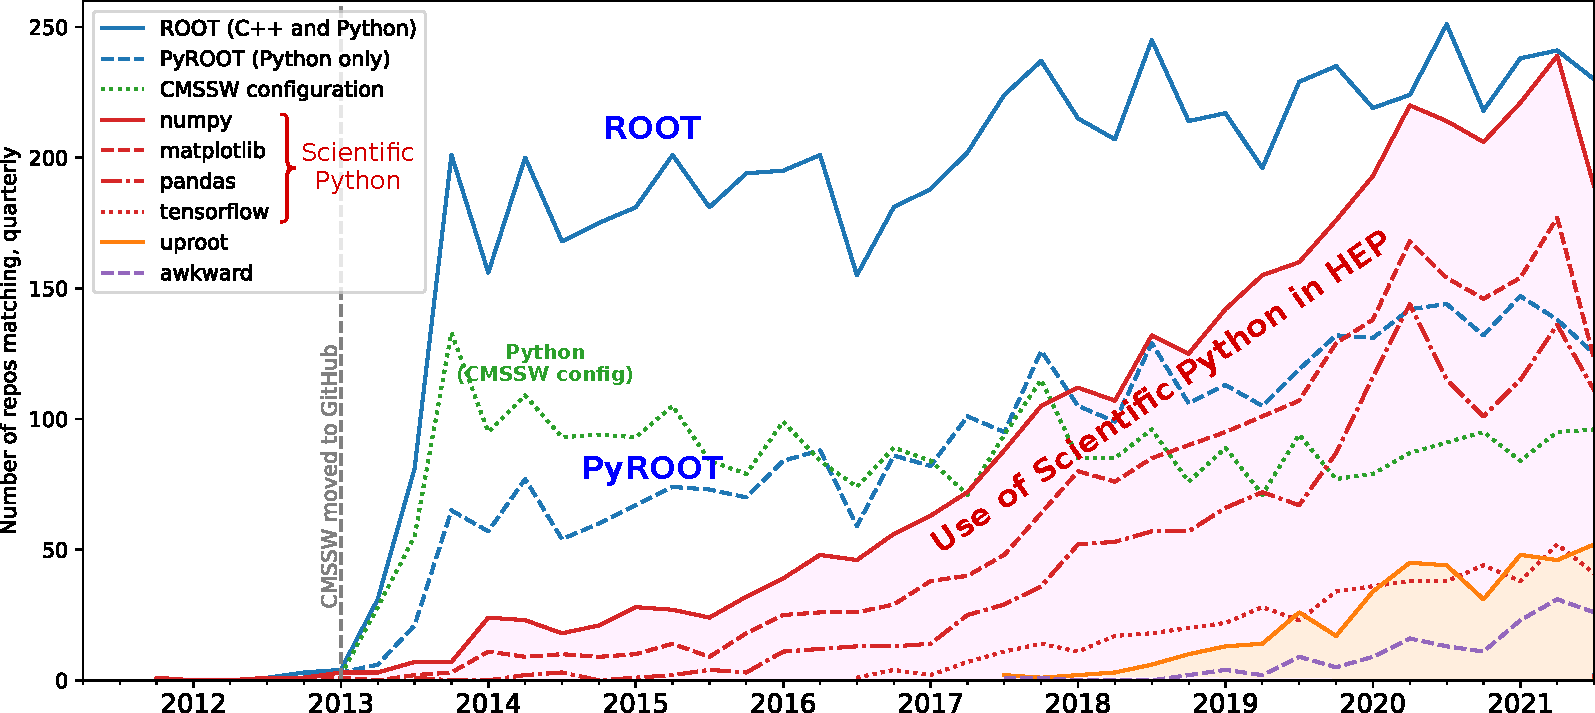
\includegraphics[width=\linewidth]{github-package-fullstudy-for-review.pdf}
\end{frame}

\begin{frame}{Another}
\vspace{0.25 cm}
\textcolor{darkblue}{Source: ``\mintinline{python}{import XYZ}'' matches in GitHub repos for users who fork CMSSW.}

\vspace{0.2 cm}
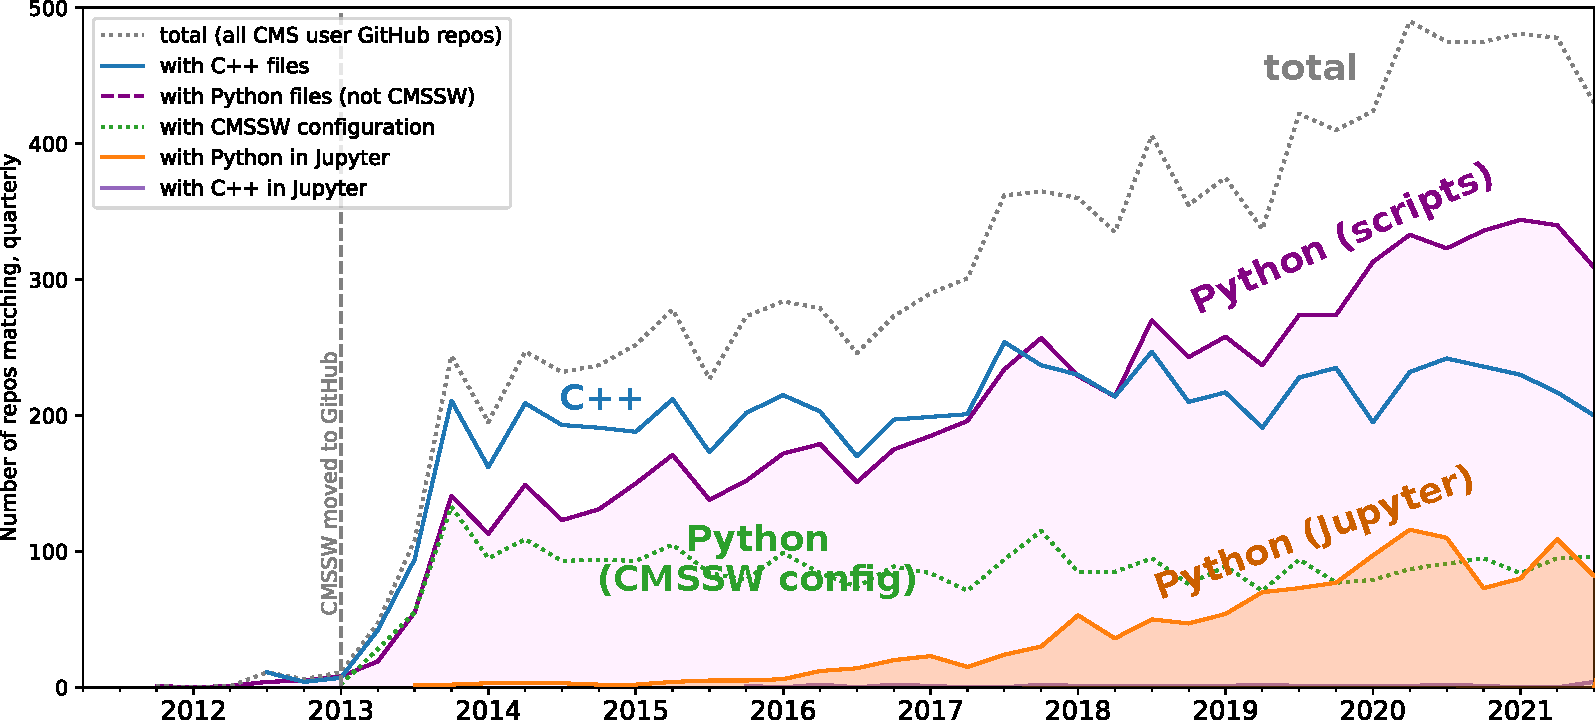
\includegraphics[width=\linewidth]{github-language-fullstudy-for-review.pdf}
\end{frame}
